\chapter{Fundamentos básicos}

Este capitulo apresenta os principais conceitos e definições necessários para o entendimento deste trabalho. A seção 2.1 apresenta definições de sistemas multiagentes
A seção 2.2 apresenta uma breve explicação sobre a arquitetura da plataforma JAMA, bem como o seu funcionamento.

\section{Sistemas Multiagentes}

\subsection{Inteligência artificial}

Antes de explicarmos o conceito de sistemas multiagentes (SMA), é necessário mostrar conceitos que são base para o entendimento de SMA. Inicia-se apresentando alguns conceitos de Inteligencia Artificial (IA). De acordo com~\cite{poole98} identificamos que a definição de IA pode variar em duas dimensões principais. Usando a definição de sistemas computacionais que agem racionalmente temos:

\begin{quote}
\emph{Computational Intelligence is the study of the design of intelligent agents.}
\end{quote}

Nessa definição, é importante ressaltar que o agente é uma entidade que atua racionalmente, esperando-se que essa racionalidade e outras características o diferencie de simples programas.

Com o crescimento dos estudos relacionado a este campo, a inteligência artificial ganhou várias áreas de atuação e resolução de problemas no nosso cotidiano. Um dos problemas é a necessidade de executar aplicações que resolvem problemas de alta complexidade. Essas aplicações podem exigir um hardware muito caro para a execução, ou então pode-se usar a abordagem de distribuí-la em vários computadores que dividem a sua execução. É justamente onde entra a inteligência artificial distribuída: São sistemas que são compostos por vários agentes coletivos, ou seja, distribuem o trabalho uns com os outros. Cada agente pode possuir uma capacidade diferente, sendo possível realizar a tarefa de modo paralelo. 

\subsection{Agente}

De acordo com~\cite{novig95}, agentes são entidades (reais ou virtuais) que funcionam de forma autônoma em um ambiente, ou seja, não necessitam de intervenção humana para realizar processamento. Esse ambiente de funcionamento do agente geralmente contém vários outros agentes e é possível a comunicação entre eles através do ambiente por meio de troca de mensagens. Em geral o funcionamento de agentes acontece de forma a perceberem o ambiente em que estão por meio de sensores, fazem análises com base nessa interação inicial e por fim podem agir sobre o ambiente de forma a modifica-lo por meio de efetuadores. A figura~\ref{fig:agente-basico} apresenta um resumo do que foi dito.

\begin{figure}
	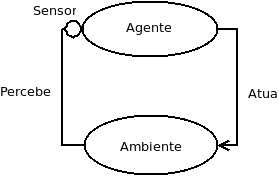
\includegraphics[scale=0.75]{images/agente-basico.png}
	\caption{Esquematização do funcionamento básico de um agente em um ambiente.}
	\label{fig:agente-basico}
\end{figure}

Agentes racionais seguem o princípio de racionalidade básico: sempre objetivam suas ações pela escolha da melhor ação possível segundo seus conhecimentos. Logo é possível inferir que a ação de um agente nem sempre alcança o máximo desempenho, sendo desempenho o parâmetro definido para medir o grau de sucesso da ação de um agente com base nos seus objetivos.

Como dito anteriormente, agentes estão presentes em um ambiente. O agente não tem controle total do ambiente, ele pode no máximo influenciá-lo com a sua atuação. Podemos separar ambientes em classes: Software, Físico e Relidade virtual (simulação de ambientes reais em software). De acordo com~\cite{wooldridge04} temos, em geral, ambientes tem propriedades inerentes que dizem respeito ao seu funcionamento:

\begin{itemize}
	\item Observável: Neste tipo de ambiente, os sensores dos agentes conseguem ter percepção completa do ambiente. Por exemplo, um sensor de movimento consegue ter visão total em um ambiente aberto.
	\item Determinística: O próximo estado do ambiente é sempre conhecido dado o estado atual do ambiente e as ações dos agentes. O oposto do ambiente determinístico é o estocástico, quando não temos certeza do estado do ambiente. Por exemplo, agentes dependentes de eventos climáticos.
	\item Episódico: A experiência do agente é dividida em episódios, onde cada episódio é a percepção do agente e a sua ação.
	\item Sequêncial: A ação tomada pelo agente pode afetar o estado do ambiente e ocasionar na mudança de estado
	\item Estático: O ambiente não é alterado enquanto um agente escolhe uma ação.
	\item Discreto: Existe um número definido de ações e percepções do agente para o ambiente em cada turno.
	\item Contínuo: As percepções e ações de um agente modificam-se em um espectro contínuo de valores. Por exemplo, temperatura de um sensor muda de forma contínua.
\end{itemize}

Na tabela~\ref{lista_agentes} mostramos alguns exemplos de agentes, apresentando as suas características já discutidas nesse trabalho.

\begin{table}
	\begin{tabular}{|p{3cm} | p{3cm} | p{2cm}| p{3cm} | p{3cm} |}
		\hline
		\textbf{Tipo de agente}	& \textbf{Medida de performance} & \textbf{Ambiente} & \textbf{Atuadores}  & \textbf{Sensores}	\\
		\hline
		Sensores de estacionamento	& Avarias no veículo & Carro e garagens & Freio do carro, controle de velocidade & Sensor de proximidade	\\
		\hline
		Jogos com oponente computador	& Quantidade de vitórias &	Software & Realizar jogada & Percepção do tabuleiro	\\
		\hline
		Agentes hospitalares		& Saúde do paciente & Paciente, ambiente médico & Diagnósticos & Entrada de sintomas do paciente	\\
		\hline
	\end{tabular}
	\caption{Listagem de sistemas multiagentes com propriedades de medida de performance, ambiente, atuadores e sensores}
	\label{lista_agentes}
\end{table}
 
A primeira linha da tabela~\ref{lista_agentes} é apresentado um exemplo de um agente atuando em um veículo como um sensor de estacionamento. Responsável por auxiliar o motorista no ato de estacionar o carro, o seu ambiente é da classe físico (considerando o carro e o ambiente onde está o carro). Seu sensor de proximidade é a percepção do ambiente e caso detecte que está próximo de um obstáculo pode atuar nos freios dos carros diminuindo a velocidade e evitando colisões. Avarias no carro podem indicar um mal funcionamento do sensor.

A última linha da tabela~\ref{lista_agentes} expõe um exemplo de um agente médico atuando em um ambiente estático um paciente. Esse ambiente é dito estático por que não será alterado pelo agente nesse exemplo, mas podendo ser diferente dependendo da aplicação. O objetivo principal é monitorar a saúde do paciênte, logo a medida de performance será a aproximação ou não do diagnóstico médico. Seu atuador não será diretamente no ambiente (corpo humano), será na forma de relatórios médicos e seus sensores podem variar de acordo com a doença a ser monitorada.

Conforme podemos encontrar em~\cite{wooldridge04}, podemos definir algumas noções gerais de agentes. A primeira, chamada de noção fraca, contém a maior parte dos agentes. Ela compreende os aspectos de \emph{reatividade}, \emph{proatividade} e \emph{habilidade social}. O conceito de reatividade  está ligado com o agente perceber o ambiente e reagir. Proatividade é a característica do agente tomar a iniciativa e agir sem a necessidade de nenhum estímulo. Habilidade social é a capacidade de interação com outros agentes.

Já a noção forte de agente envolve os seguintes aspectos: , veracidade, benevolência
\begin{itemize}
	\item Mobilidade: O Agente deve pode mover-se no ambiente, por exemplo, em uma rede.
	\item Veracidade: Agente não comunica informações falsas.
	\item Benevolência: Agente ajudará os outros.
	\item Racionalidade: O agente não irá agir de forma a impedir a realização de seus objetivos.
	\item Cooperação: O agente coopera com o usuário.
\end{itemize}

\subsection{Arquitetura de agentes}

A arquitetura de agentes varia de acordo com a complexidade da sua autonomia, ou seja, com a capacidade de reagir aos estímulos do ambiente. Conforme verificado no livro de ~\cite{novig95}, os tipos de arquitetura são: orientadas à tabela, reflexiva simples, reflexiva baseado em modelo, baseada em objetivo, baseada em utilidade.

A primeira arquitetura a ser explorada é o agente orientado à tabelas. Todas as ações dos agentes dessa arquitetura são conhecidas e estão gravadas em uma tabela. Assim, quando o agente receber o estímulo ele já terá a ação a ser tomada previamente gravada em sua memória. Logo para construir esse tipo de agente, fica claro que além de saber todas percepções possívels, será necessário definir ações apropriadas para todas. Isso levará a tabelas muito complexas e o tamanho pode facilmente passar a ordem de milhões dependendo do número de entradas.

A arquitetura reflexiva simples é um dos tipos mais simples de agente. Nele, o agente seleciona a ação com base unicamente na percepção atual, desconsiderando assim uma grande tabela de decisões. A decisão é tomada com base de regras condição-ação: Se uma condição ocorrer, uma ação será tomada. Por exemplo, vamos supor um agente médico que determina o diagnóstico de uma doença no paciente caso exista alguma anomalia no organismo (Por exemplo, paciente com febre). Uma condição-ação poderia ser:

if anomalia-organismo then diagnóstico-médico

Esse tipo de agente é bastante simples, o que é uma vantagem comparado à arquitetura de tabela. Porém, essa abordagem requer um ambiente totalmente observável, visto que esse tipo de agente possui uma inteligência bastante limitada. No exemplo do agente médico existem diversas maneiras de se detectar uma anomalia no organismo do paciente, seria necessário conhecer todas as formas para usarmos uma abordagem reativa simples.

A arquitetura reflexiva baseada em modelos funciona de maneira similar a anterior. Nessa abordagem, é levado em conta a parte do ambiente que não é visível neste momento. E para saber o ``momento atual'' de um agente, é necessário guardar a informação de estado consigo. Para atualizar o estado do agente, é necessário conhecer como o mundo desenvolve-se independente do agente (no caso do exemplo, como o organismo funciona) e é necessário saber as ações dos agentes no ambiente. Esses dois conhecimentos do ambiente são chamados de \textbf{modelo do mundo}. O agente que usa esse tipo de abordagem é chamado de agente baseado em modelo.

Na arquitetura reflexiva baseada em objetivo, as ações do agente são tomadas apenas se o aproximam de alcançar um objetivo. Para isso, será necessário algo além do estado atual do ambiente: Será necessário informações do objetivo a ser atingido. Assim o agente pode combinar as informações do estado e o objetivo para determinar se deve ou não agir sobre o ambiente. Essa arquitetura porém é obviamente mais complexa e de certa forma ineficiente. Porém ela permite uma maior flexibilização das ações em determinados ambientes, visto que suas decisões são representadas de forma explícita e podem ser modificadas. É interessante notar que esse tipo de arquitetura não trata ações com objetivos conflitantes.

E por fim, a arquitetura reflexiva baseada em utilidade não utiliza apenas objetivos para realizar a próxima decisão, mas dá ao agente a capacidade de fazer comparações sobre o estado do ambiente e as ações a serem tomadas: Quais delas são mais baratas, confiáveis, baratas, rápidas do que as outras. A capacidade de avaliação do agente chama-se função de utilidade, que mapeia uma sequência de estados em um número real que determina o grau de utilidade. Esse mecanismo possibilita a decisão racional de escolha entre vários objetivos conflitantes. Por exemplo, escolher entre um objetivo mais barato ao invés de escolher entre o mais rápido.

\subsection{Sistemas Multiagentes}

Sistemas multiagentes são sistemas compostos por vários agentes capazes de se comunicar, possuindo uma linguagem de alto nível para isso. O agente deve ser conhecimento para realizar uma determinada tarefa e pode ou não cooperar com outros agentes para realizá-la.

Fica claro nessa definição que sistemas multiagentes

De acordo com~\cite{sarmento11}, podemos encontrar as seguintes características principais de ambientes em SMAs:
\begin{itemize}
	\item Ambientes SMAs fornecem protocolos específicos para comunicação e interação. Cada ambiente tem as suas particularidades: Alguns são em uma única máquina, outros são compartilhados com o mundo real e outros são distribuídos. Cabe a cada ambiente definir um protocolo onde todos agentes devem obedecer para comunicar-se.
	\item SMAs são tipicamente abertos.
	\item SMAs contém agentes que são autônomos e individualistas.
\end{itemize}

\section{Dependabilidade}


Antes de falar em dependabilidade, é necessário algumas definições.

A definição original de dependabilidade de software é a habilidade de um sistema prover um serviço que pode ser justificadamente confiável. Uma outra definição alternativa é a dependabilidade de um sistema é a habilidade de evitar falhas que são mais frequentes e mais graves do que o aceitável.

Dependabilidade é uma área que vem desenvolvendo seus estudos de forma crescente ao longo dos anos. De acordo com~\cite{algirdas04}, o conceito de dependabilidade abrange uma série de principais atributos que a integram. O primeiro deles é disponibilidade, onde um serviço deve estar o disponível o máximo de tempo possível. A confiabilidade garante que o serviço usado é sempre confiável. A segurança é a garantia de não haver consequências catastróficas para o ambiente no uso do serviço. Integridade garante não alteração nas propriedades. Manutenibilidade é a garantia que é possível mudanças e reparos no sistema provedor do serviço.

Alguns atributos são muito próximos da segurança da informação, como por exemplo a confidencialidade, que é a capacidade de não prover informação para entidades desconhecidas. Outros atributos são, na verdade, uma composição com a segurança. Por exemplo a integridade e disponibilidade. Integridade com acessos não autorizados e disponibilidade apenas para acessos autorizados. A figura~\ref{fig:dependabilidade-seguranca} sintetiza o que foi dito, mostrando os atributos em comum das duas áreas:

\begin{figure}
	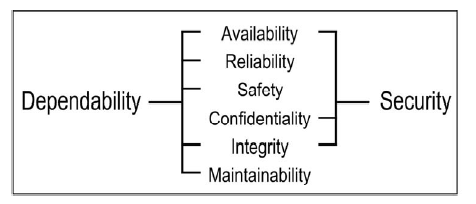
\includegraphics[scale=0.75]{images/dependabilidade-seguranca.png}
	\caption{Dependabilidade, segurança e seus atributos em comum. Fonte:~\cite{algirdas04}}
	\label{fig:dependabilidade-seguranca}
\end{figure}

Dado que sistemas começam a ser modelados a partir de especificações de componentes, os desafios de dependabilidade hoje para estudos futuros são muitos. O primeiro deles é determinar precisamente a qualidade desses atributos de forma precisa, sabendo que são especificados de forma imprecisa. É necessário também determinar em que medida e quais restrições as propriedades emergentes podem ser derivadas das propriedades de um sistema. E dado um conjunto de propriedades, quais delas são previsíveis.

Mais especificamente, em um sistema multiagente, é a propriedade que podemos medir sobre a confiança que podemos mensurar em um agente dado que ele roda em um ambiente descentralizado. Devido a complexidade do ambiente, existem diversos desafios de acordo com~\cite{hoffman08} no projeto desse ambiente. Em~\cite{algirdas04} são definidos as principais propriedades relacionadas a dependabilidade, sendo um dos objetivos deste trabalho a identificação destas propriedades na plataforma JAMA.

\section{Sistemas Distribuídos}

Para o prosseguimento desse trabalho, faz-se necessário uma breve introdução a sistemas distribuídos, mais especificamente, redes \emph{peer-to-peer}(P2P). Redes P2P são diferentes do modelo cliente/servidor desde o seu funcionamento até detalhes mais complexos.

O conceito de redes P2P já existe a muito tempo, porém com o aparecimento da Rede Napster essa tecnologia, essa tecnologia ganhou mais atenção mundial. Diversos estudos de redes P2P foram surgindo, como por exemplo arquitetura , segurança, etc.

O objetivo geral dessa seção é explicar as principais definições de tecnologias usadas pela rede P2P para o entendimento da plataforma JAMA.

\subsection{Introdução}

As redes peer to peer surgem como uma forma alternativa ao funcionamento do modelo cliente servidor. A principal diferença entre essas abordagens é que no modelo cliente/servidor, uma das entidades (servidor) é responsável por prover um recurso na rede para que outras entidades (clientes) possam consumi-lo. Se o servidor não possuir o recurso ou ele deixar de existir, os seus clientes ficam impossibilitados de usar o recurso, a menos que exista outro servidor na rede.

Já o sistema P2P possui princípios de funcionamento diferente. De acordo com a definição de P2P encontrada em~\cite{rudiger02}:

\begin{quote}
A distributed network architecture may be called a Peer-to-Peer (P-to-P, P2P,...) network, if the participants share a part of their own hardware resources (processing power, storage capacity, network link capacity, printers,...). These shared resources are necessary to provide the Service and content offered by the network (e.g. file sharing or shared workspaces for collaboration). They are accessible by other peers directly, without passing intermediary entities. The participants of such a network are thus resource (Service and content) providers as well as resource (Service and content) requestors (Servent-concept).
\end{quote}

Ou seja, em redes P2P os participantes (par) possuem ambas as funcionalidades de cliente e servidor: Eles disponibilizam recursos na rede (Hardware, processamento, arquivos) que podem ser disponibilizados para outros pares que o acessam diretamente, desempenhando assim o papel de servidor. Simultaneamente, esse mesmo par pode requisitar recursos de outros pares, acessando diretamente e desempenhando assim o papel de cliente. Dessa forma, os pares dessa rede são ao mesmo tempo cliente e servidor.

Alguns autores atribuem	o nome P2P à rede Napster devido à explosão do seu acesso (ano 2000). É importante ressaltar que os estudos de Peer-to-peer é bem mais antigo, sendo possível encontrar aplicações mais antigas. A internet por exemplo surge como um sistema P2P que permite o compartilhamento de recursos entre computadores nos Estados Unidos.

Podemos citar também o DNS, que faz um mapeamento entre nomes de domínios e endereços IPs. De acordo com~\cite{stevens93}, o DNS age como um banco de dados distribuído que armazena nomes de \emph{hosts} e seus respectivos endereços ip. É dito distribuído por que não é um site que contém o conhecimento desses dados. Basicamente, quando um \emph{host} é perguntado sobre um endereço, ele pode repassar para outros \emph{hosts} que tenham o conhecimento caso não seja possível encontrar em seu banco de dados. Dessa forma, a informação é descentralizada e mecanismos de redundância são mais fáceis de existir.

Em meados de 1999 quando Shawn Fanning, na época estudante de 18 anos, criou um programa para compartilhamento de músicas usando rede P2P como uma ferramenta para atingir seu objetivo. De acordo com~\cite{oram01} essa aplicação não era totalemente descentralizada. Segundo a mesma referência, o funcionamento se dava da seguinte forma: Existia um repositório central onde eram armazenadas informações de quas músicas os pares tinham. Cada par que quisesse fazer uma busca consultava o repositório, conectava-se diretamente ao par e transferia a música. Essa característica é ainda de modelo servidor, porém os pares da rede podiam agir de forma a disponibilizar músicas ou requisitar músicas simultaneamente, deixando a disponibilização de músicas descentralizadas.

O Napster porém foi acusado de violação de direitos autorais pela \emph{Recording Industry Association of America} (RIAA). Após uma longa batalha judicial, um acordo foi feito obrigado o Napster a pagar dezenas de milhões para autores e gravadoras. Essa foi o início da decadência do Napster, deixando de existir em 2003 e sendo comprado pela \emph{Roxio}, mudando o seu modelo de funcionamento.

A tecnologia P2P então evoluiu muito rápido devido ao sucesso do Napster. A rede P2P evolui de forma a não permitir apenas compartilhamento de músicas, porém qualquer tipo de dado. Outras programas e arquiteturas foram surgindo com o passar do tempo, como por exemplo o \emph{{K}a{Z}aa} e o \emph{Gnutella}. Essas redes desenvolveram uma arquitetura completamente descentralizada, dificultando ainda mais o controle de fluxo na rede.

O P2P atualmente não tem seu grande fim apenas no compartilhamento de conteúdo multimídia. Diversas aplicações corporativas fazem uso de uma rede descentralizada objetivando desempenho, tempo de resposta, redução de recursos, dentre outros. Supondo apl

\subsection{Arquitetura}

\subsection{Roteamento}

\section{JAMA}

O desenvolvimento completo da plataforma JAMA está descrita em~\cite{parise11}. Seu objetivo foi desenvolver uma plataforma de sistemas multiagentes distruibuído e com fraco acoplamento entre os agentes e as camadas mais baixas do sistemas, permitindo assim o desenvolvimento de novas funcionalidades. Essa nova plataforma garante a comunicação dos agentes com as outras entidades do ambiente. Atualmente o JAMA está somente com a parte de comunicação de serviços funcional, necessitando de implementação na parte de suporte a agentes.

O JAMA foi desenvolvido na linguagem Java e outros frameworks de softwares distrubuidos. Basicamente foi usado tecnologias como o Google Guice (pronunciado juice), que trabalha com injeção de dependências e garante que o código não precise criar objetos diretamente, reduzindo então a dependencia de ``fábricas'' de criações de objetos.

Por se tratar de uma plataforma de sistemas distribuídos, foi necessário escolher um protocolo de rede para a implementação. O protocolo escolhido foi o Peer-to-peer (P2P) pois oferecem uma série de propriedades interessantes para a aplicação:
\begin{itemize}
	\item Tolerância a falhas.
	\item Balanceamento de carga.
	\item Escalabilidade da aplicação.
	\item Descentralização dos serviços nas bordas da rede	.
\end{itemize}

Como foi dito anteriormente, um sistema multiagente tem basicamente duas entidades: Agentes e o ambiente. A plataforma JAMA procurou fazer do ambiente o componente principal no desenvolvimento. Logo a sua arquitetura basicamente preocupou-se com as duas entidades listadas anteriormente e outros dois componentes: Barramento de eventos e um adaptador de rede, visto que é uma aplicação distribuída.

\subsection{Ambiente}

Na arquitetura do JAMA atua como uma camada que abstrai as camadas inferiores, permitindo a localização e comunicação de agentes de forma mais transparente. Os agentes emitem mensagens nesse ambiente e ele se encarrega de notificar todos os agentes ouvintes. Por ser uma arquitetura distribuída, os agentes não tem conhecimento se estão rodando na mesma máquina ou não. Logo não existe comunicação direta entre os agentes, o ambiente será o mediador entre eles caso seja necessário haver algum tipo de comunicação. A imagem~\ref{fig:ambiente} sintetiza o que foi explicado.

\begin{figure}
	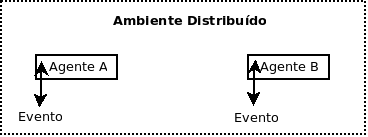
\includegraphics[scale=0.75]{images/ambiente.png}
	\caption{Ambiente distriuído no JAMA. Os agentes não se comunicam diretamente.}
	\label{fig:ambiente}
\end{figure}

O ambiente do JAMA é capaz também de atuar como plataforma provedora de serviços. Aplicações como banco de dados distribuídos, transporte de agentes, e outros podem estar disponíveis na plataforma, bastando apenas serem registrados para serem encontrados pelos agentes. Esses serviços em sua grande maioria são suporte para o processamento dos agentes. Em~\cite{parise11} podemos ver um exemplo de agente que usa aplicações registradas no JAMA:

\begin{quote}
Em aplicações forenses, é muito comum o uso de soluções multiagentes devido ao grande volume de dados e processamento na análise de um caso. Nestas aplicações, o ambiente desempenharia uma função importante ao prover serviços como sistema de arquivos, onde os dados seriam carregados; banco de dados distribuídos, onde os agentes submeteriam seus resultados; e uma aplicação Web, onde os usuários poderiam acompanhar o andamento da análise e executar ações sobre o sistema. Os agentes ficariam com a única responsabilidade de se organizar e executar o trabalho utilizando os serviços fornecidos.
\end{quote}

\subsection{Adaptador de rede}

O Adaptador de rede é responsável por integrar os protocolos de redes ao ambiente. O adaptador de rede deve possuir funcionalidades básicas implementadas para uso da plataforma. Como o JAMA foi projetado para fazer uso de um \emph{middleware open-source} que já implementasse as funcionalidades básicas, não foi necessário fazer uma implementação do início. O \emph{middleware peer-to-peer pastry} foi escolhido para a implementação pois possui bom suporte a segurança, mensagens multicast e boa documentação disponível na internet.

O adaptador é funciona de forma a receber eventos das camadas superiores, serializa os eventos em uma mensagem de rede e envia para a aplicação em algum lugar na rede. Ao receber a mensagem, ela é \emph{desserializada} em um evento e este evento é enviado para as camadas superiores.

\subsection{Barramento de eventos}

O JAMA foi definido para funcionar com o sistema de eventos: Toda e qualquer comunicação entre agentes é feita desta forma. Dessa forma a aplicação não fica acoplada a um tipos específicos de objetos, aumentando assim a escalabilidade da aplicação.

O sistema de eventos está ligado com a definição de evento e ouvintes. Ao montar-se um evento, são passandas todas as informações que forem jugadas necessárias para a comunicação. Em seguida o evento é enviado e a plataforma notifica apenas os ouvintes que estão interessados em receber a comunicação.

O sistema que implementa o despacho e a notificação de eventos é o sistema de barramentos. Seu projeto foi orientado a ser implementado em três padrões de projetos. O primeiro padrão é o \emph{Singleton}, pois o barramento deve ser único na aplicação. O segundo padrão é o \emph{Observer}, pois é nele que se encontram os registros dos ouvintes do sistema e ele irá notifica-los dos eventos enviados. O terceiro padrão é o \emph{Mediator} pois ele atua como mediador da comunicação de elementos da plataforma.

\subsection{Agente}

A parte de agente é responsável por implementar a lógica de sistemas multiagentes. No JAMA, os agentes são executados em paralelo através de Threads separados, sendo responsáveis pelo seu estado e seu fluxo de execução.

O ciclo de vida de um agente segue basicamente os seguintes passos:

\begin{itemize}
	\item \emph{Start} - Ao criar o agente, o ciclo start é iniciado. Normalmente é usado para configurações iniciais do agente.
	\item \emph{Loop} - Código principal que é executado no agente.
	\item \emph{Sleep} - Interrupção da atividade do agente, podendo ser acordado no futuro.
	\item \emph{Wakeup} - Volta para o estado ativo e continua a execução do trecho \emph{loop}.
	\item \emph{Destroy} - Destrói a instância do agente, finalizando a execução.
\end{itemize}


\section{Desafios desse trabalho}
O trabalho porém carece de uma análise de dependabilidade, envolvendo os seus componentes e integração dos mesmos. Não existe um estudo detalhado mensurando o grau de dependabilidade entre os componentes principais (barramento de eventos, adaptador de rede, serviços da rede, etc), nem mesmo detalhando a dependência entre esses módulos. Faz-se necessário então um estudo mais aprofundado na plataforma, sendo esse portanto o foco principal deste trabalho.



























